\documentclass[10pt, a4paper]{article}
\usepackage[T2A]{fontenc}
\usepackage[english, russian]{babel}

\usepackage{graphicx}
\graphicspath{{./figs/}}

\usepackage{amsmath}
\usepackage{amssymb}
\usepackage{mathtools}
\usepackage{physics}
\usepackage{upgreek}
\usepackage{sectsty}
\usepackage{color,soul}
\usepackage[colorlinks=true,allcolors=blue]{hyperref}
\sectionfont{\centering}

\usepackage{geometry}
 \geometry{
 a4paper,
 margin=25mm,
 }

\title{Билеты к кандидатскому экзамену по физике плазмы}
\date{}

\begin{document}

\newpage
\section{Термодинамика плазмы}
\label{sec.1}

\subsection{Понятие плазмы, квазинейтральность, микрополя, дебаевский радиус, идеальная и неидеальная плазма.}
\label{sec.1.1}

Плазма - это частично или полностью ионизированный газ, в котором меются следующие свойства  - наличие радиуса дебая 
($r_d=\left(\frac{T}{8\pi n e^2}\right)^2$), наличие ленгмюроовских волн (или плазменных волн, их можно рассматривать,
как колебания слоя электронов относительно ионов на частоте $\omega_p^2=\frac{4\pi n e^2}{m}$), а так же затухания Ландау. 

У плазмы вводят т.н. параметр неидеальности, который есть $g = \frac{1}{n * r_d^3}$(Kroll, eq. 1.3.1). Когда 
$g \ll 1$ говорят, что плазма идеальна, т.к. в этом случае её свойства, как газа, схожи с идеальным газом.





~\cite{kotelnikov}. Ссылка на уравнение~\eqref{eq.Euler}, Рис.~\ref{fig.1.2.1}.


\begin{equation}
    \label{eq.Euler}
    e^{i \pi} + 1 = 0
\end{equation}

\subsection{Условие термодинамического равновесия, термическая ионизация, формула Саха, корональное равновесие, снижение потенциала ионизации.}
\label{sec.1.2}

Картинка

\begin{figure}[h!]
    \center{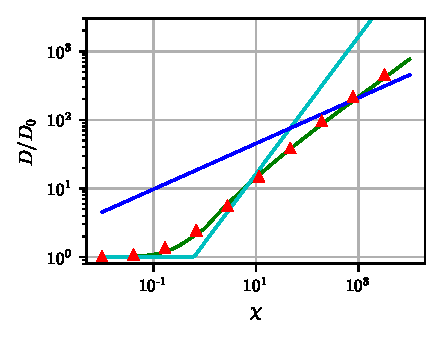
\includegraphics[width=85mm]{test.pdf}}
    \caption{\label{fig.1.2.1} Подпись.}
\end{figure}

\subsection{Вырождение плазмы, статистика Больцмана и Ферми—Дирака, модель Томаса—Ферми.}

Плазма

\newpage
\addcontentsline{toc}{section}{Список литературы}
\bibliographystyle{unsrt}
\bibliography{program}

\end{document}
